
\setcounter{chapter}{8}

\chapter{Feedback and Sensitivity}
\label{ch:feedback_sensitivity}

\begin{quote}
\textit{``I suddenly realized that if I fed the amplifier output back to the input, in reverse phase, and kept the device from oscillating, I would have exactly what I wanted: a means of canceling out the distortion in the output.''}

\hfill --- Harold S. Black, 1927
\end{quote}

\vspace{1em}

\noindent The principle of negative feedback stands as one of the most profound engineering insights of the twentieth century. In this chapter, we explore how feeding back a portion of a system's output to its input---seemingly a wasteful process that ``throws away'' gain---actually provides remarkable benefits: rejection of disturbances, reduction of sensitivity to component variations, and predictable system behavior despite uncertain plant dynamics. These properties make feedback the cornerstone of modern control system design.

%=============================================================================
\section{Historical Motivation: The Birth of Negative Feedback}
\label{sec:historical_motivation}
%=============================================================================

\subsection{The Telephone Amplifier Problem}

In the early decades of the twentieth century, the American Telephone \& Telegraph Company (AT\&T) faced a formidable engineering challenge. As telephone networks expanded across the continental United States, voice signals had to traverse thousands of miles of copper wire. The inherent resistance of these transmission lines caused severe signal attenuation---a coast-to-coast call required amplification by a factor of approximately $10^{30}$ to maintain intelligible speech \cite{black1934}.

The solution appeared straightforward: cascade multiple vacuum tube amplifiers along the transmission path. A transcontinental line might employ 50 to 100 amplifier stations, each providing gains of 20 to 40 decibels. However, this approach encountered two devastating problems that threatened the viability of long-distance telephony.

\begin{figure}[htbp]
\centering
\begin{tikzpicture}[scale=0.9]
    % Transmission line with amplifier stations
    \draw[thick] (0,0) -- (12,0);

    % Amplifier stations
    \foreach \x/\n in {1/1, 3/2, 5/3, 7/..., 9/49, 11/50} {
        \draw[fill=gray!30] (\x-0.3,-0.4) rectangle (\x+0.3,0.4);
        \node[font=\tiny] at (\x,0) {Amp};
        \node[font=\tiny, below] at (\x,-0.6) {\n};
    }

    % Input and output
    \node[left] at (0,0) {New York};
    \node[right] at (12,0) {San Francisco};

    % Signal levels
    \draw[->,thick,blue] (0,1.2) -- (1,1.2);
    \node[above,font=\small,blue] at (0.5,1.2) {Input};

    % Gain arrows
    \draw[->,thick,red] (1.5,0.8) -- (2.5,1.3);
    \draw[->,thick,red] (3.5,0.8) -- (4.5,1.3);

    % Distortion accumulation
    \draw[decorate, decoration={snake, amplitude=1mm, segment length=3mm}, thick, orange]
        (6,1.5) -- (9,1.5);
    \node[above,font=\small,orange] at (7.5,1.6) {Distortion accumulates};

    % Temperature variation
    \draw[<->,thick,purple] (2,-1.2) -- (4,-1.2);
    \node[below,font=\small,purple] at (3,-1.2) {$\pm 20\%$ gain drift};
\end{tikzpicture}
\caption{The transcontinental telephone amplifier chain. Each amplifier station introduced gain variations due to temperature changes and component aging, and nonlinear distortion that accumulated through the cascade.}
\label{fig:telephone_chain}
\end{figure}

\textbf{Problem 1: Gain Instability.} Vacuum tube amplifiers exhibited significant gain variations with temperature, power supply fluctuations, and component aging. A single amplifier might drift by $\pm 10\%$ to $\pm 20\%$ over its operating conditions. When fifty such amplifiers were cascaded, the cumulative gain uncertainty became catastrophic. If each amplifier's gain $A_i$ varied by a factor $(1 + \epsilon_i)$ where $|\epsilon_i| \leq 0.1$, the total gain varied as:
\begin{equation}
A_{\text{total}} = \prod_{i=1}^{50} A_i(1 + \epsilon_i) \approx A_{\text{nominal}} \prod_{i=1}^{50}(1 + \epsilon_i)
\end{equation}

For independent variations, this product could easily range from $0.01$ to $100$ times the nominal value---a completely unacceptable $40$ dB uncertainty.

\textbf{Problem 2: Distortion Accumulation.} Vacuum tubes are inherently nonlinear devices. Each amplifier introduced harmonic distortion, typically 1\% to 5\% total harmonic distortion (THD). Through a cascade of amplifiers, distortion products were re-amplified and new distortion was added, resulting in unintelligible speech at the receiving end. The distortion in a cascade grows roughly as:
\begin{equation}
\text{THD}_{\text{total}} \approx \sqrt{\sum_{i=1}^{N} \text{THD}_i^2} \quad \text{(for uncorrelated distortion)}
\end{equation}

With 50 amplifiers each contributing 2\% THD, the total approached 14\%---rendering speech quality unacceptable.

\subsection{Harold Black's Revolutionary Insight}

Harold Stephen Black (1898--1983) joined Bell Telephone Laboratories in 1921 and was assigned to the repeater amplifier problem. For six years, he pursued conventional approaches: improving vacuum tube linearity, using push-pull configurations to cancel even harmonics, and developing sophisticated matching networks. Progress was incremental and insufficient.

The breakthrough came on the morning of August 2, 1927, during Black's commute on the Lackawanna Ferry crossing the Hudson River from New Jersey to Manhattan. In a flash of insight, Black conceived of an entirely different approach: rather than trying to build a perfect amplifier, he would use feedback to force an imperfect amplifier to behave as if it were nearly ideal.

Black's key insight was captured in a sketch he made on a page of the \textit{New York Times} that morning---a diagram that would become one of the most important figures in engineering history:

\begin{figure}[htbp]
\centering
\begin{tikzpicture}[auto, node distance=2cm, >=latex']
    % Blocks
    \node[draw, circle, minimum size=0.6cm] (sum) at (0,0) {$\Sigma$};
    \node[draw, rectangle, minimum width=1.5cm, minimum height=1cm, fill=blue!20] (amp) at (3,0) {$\mu$};
    \node[draw, rectangle, minimum width=1.2cm, minimum height=0.8cm, fill=green!20] (beta) at (3,-2) {$\beta$};

    % Input/output
    \node[left] at (-2,0) {$V_{in}$};
    \node[right] at (5.5,0) {$V_{out}$};

    % Arrows
    \draw[->] (-2,0) -- (sum);
    \draw[->] (sum) -- node[above] {$\epsilon$} (amp);
    \draw[->] (amp) -- (5,0);
    \draw[->] (5,0) -- (5.5,0);

    % Feedback path
    \draw[->] (5,0) -- (5,-2) -- (beta);
    \draw[->] (beta) -- (0,-2) -- (sum);

    % Signs
    \node[font=\small] at (-0.3,0.3) {$+$};
    \node[font=\small] at (-0.3,-0.4) {$-$};

    % Labels
    \node[below] at (3,0.5) {High-gain amplifier};
    \node[below] at (3,-2.5) {Feedback network};
\end{tikzpicture}
\caption{Black's negative feedback amplifier concept, as sketched on the ferry in 1927. The amplifier gain $\mu$ is intentionally made very large, while the feedback network $\beta$ is constructed from stable, precise passive components.}
\label{fig:black_original}
\end{figure}

The mathematics Black developed were elegantly simple. Let $\mu$ be the open-loop amplifier gain and $\beta$ be the feedback factor. The closed-loop gain becomes:
\begin{equation}
A_f = \frac{\mu}{1 + \mu\beta}
\label{eq:black_formula}
\end{equation}

When the \textit{loop gain} $\mu\beta \gg 1$, this reduces to:
\begin{equation}
A_f \approx \frac{\mu}{\mu\beta} = \frac{1}{\beta}
\label{eq:black_approximation}
\end{equation}

This was Black's revolutionary insight: \textbf{the overall gain depends only on the feedback network $\beta$, not on the amplifier gain $\mu$}. The feedback network could be constructed from precision resistors---passive components that are inherently stable with temperature, aging, and manufacturing variations. The vacuum tube's gain could vary wildly, yet the system's gain would remain rock-steady.

\subsection{The Patent Battle and Initial Skepticism}

Black's patent application, filed in 1928, met with unprecedented resistance. Patent examiners refused to believe that an engineer would deliberately ``throw away'' gain---the hard-won gain that vacuum tube designers had struggled for years to achieve. The application spent nine years in the Patent Office before U.S. Patent 2,102,671 was finally granted on December 21, 1937.

The skepticism was understandable. Consider an amplifier with $\mu = 10{,}000$ (80 dB). If we apply negative feedback with $\beta = 0.01$, the loop gain is $\mu\beta = 100$, and the closed-loop gain becomes:
\begin{equation}
A_f = \frac{10{,}000}{1 + 100} \approx 99
\end{equation}

The gain has been reduced by a factor of 101---from 80 dB to a mere 40 dB! Engineers at the time viewed this as absurd waste. What Black understood, and eventually convinced others of, was that this sacrifice purchased something invaluable: \textit{predictability and linearity}.

\subsection{The Mathematical Framework: Nyquist and Bode}

Black's invention worked brilliantly in practice, but a complete theoretical foundation was needed. Two of Black's colleagues at Bell Labs rose to this challenge.

\textbf{Harry Nyquist} (1889--1976) developed the stability criterion that bears his name. His 1932 paper established when a feedback system would oscillate and when it would remain stable, based on the frequency response of the loop gain $\mu\beta$. The Nyquist stability criterion provided engineers with a rigorous method to design feedback systems with guaranteed stability margins.

\textbf{Hendrik Wade Bode} (1905--1982) created the logarithmic frequency response plots (Bode plots) that made feedback system design practical. His 1945 book \textit{Network Analysis and Feedback Amplifier Design} codified the design techniques that remain in use today. Bode also established fundamental limitations on feedback system performance, including the famous ``Bode sensitivity integral'' that we will encounter later in this chapter.

Bode introduced the concept of \textit{sensitivity} as a quantitative design specification. Rather than simply noting that feedback reduced gain variations, Bode defined a mathematical function that precisely captured how much parameter variations were attenuated:
\begin{equation}
S^{A_f}_{\mu} = \frac{\partial A_f / A_f}{\partial \mu / \mu} = \frac{1}{1 + \mu\beta}
\end{equation}

This sensitivity function became a cornerstone of modern control theory.

\subsection{Impact on Telecommunications and Beyond}

The negative feedback amplifier transformed telecommunications. By 1937, transcontinental telephone service with acceptable quality became routine. The same principle was rapidly applied across the electronics industry: radio transmitters and receivers adopted feedback for improved fidelity, public address systems gained immunity to microphone placement variations, and recording and playback equipment achieved the linearity necessary for high-quality audio reproduction. The operational amplifier, which would later become the workhorse of analog computing and signal processing, relied fundamentally on feedback to achieve its remarkable versatility. During World War II, feedback-based servo mechanisms enabled the precise radar tracking and gun control systems that proved decisive in military applications.

The concepts of feedback, sensitivity, and stability that Black, Nyquist, and Bode developed for telephone amplifiers became the foundation of classical control theory. Every autopilot, every robotic arm, every temperature controller, and every power supply built since then owes a debt to that morning sketch on the Lackawanna Ferry.

%=============================================================================
\section{Modern Applications of Feedback for Sensitivity Reduction}
\label{sec:modern_applications}
%=============================================================================

The principles discovered by Black, Nyquist, and Bode permeate modern engineering. Here we survey several applications where feedback's ability to reject disturbances and reduce sensitivity is essential.

\subsection{Operational Amplifier Circuits}

The integrated circuit operational amplifier (op-amp) is perhaps the purest embodiment of Black's vision. A modern op-amp like the LM741 has an open-loop gain of approximately $\mu = 200{,}000$ (106 dB), but this gain varies significantly with temperature, loading, and frequency. In the classic inverting amplifier configuration with feedback resistors $R_1$ and $R_f$:
\begin{equation}
A_f = -\frac{R_f}{R_1} \cdot \frac{1}{1 + (R_1 + R_f)/(R_1 \mu)}
\end{equation}

When $\mu$ is large, $A_f \approx -R_f/R_1$---determined entirely by the resistor ratio. Precision resistors with $0.1\%$ tolerance yield amplifiers with $0.1\%$ gain accuracy, despite the op-amp's gain varying by factors of 2 or more.

\subsection{Voltage Regulators}

Linear voltage regulators (e.g., the LM7805) use feedback to maintain constant output voltage despite variations in input voltage (line regulation) and load current (load regulation). The pass transistor's gain varies with temperature and current, yet the output voltage remains within 1-2\% of nominal. Switching regulators employ feedback loop gains of $10^4$ or more to achieve load regulation below $0.1\%$.

\subsection{Cruise Control}

Automotive cruise control illustrates disturbance rejection. The ``plant'' is the vehicle dynamics; the ``disturbance'' is road grade (hills), wind, and rolling resistance variations. Without feedback, a fixed throttle position would cause speed to decrease on uphills and increase on downhills. With feedback from a speed sensor, the controller adjusts throttle to maintain constant speed despite these disturbances.

\begin{figure}[htbp]
\centering
\begin{tikzpicture}[auto, node distance=2cm, >=latex']
    \node[draw, circle, minimum size=0.6cm] (sum1) at (0,0) {$\Sigma$};
    \node[draw, rectangle, minimum width=1.5cm, minimum height=0.8cm] (controller) at (2.5,0) {Controller};
    \node[draw, circle, minimum size=0.6cm] (sum2) at (5,0) {$\Sigma$};
    \node[draw, rectangle, minimum width=1.5cm, minimum height=0.8cm] (vehicle) at (7.5,0) {Vehicle};

    % Labels
    \node[above] at (-1.5,0) {$v_{set}$};
    \node[above] at (5,1) {Disturbance $d$};
    \node[above] at (9.5,0) {$v_{actual}$};

    % Arrows
    \draw[->] (-1.5,0) -- (sum1);
    \draw[->] (sum1) -- (controller);
    \draw[->] (controller) -- (sum2);
    \draw[->] (5,1) -- (sum2);
    \draw[->] (sum2) -- (vehicle);
    \draw[->] (vehicle) -- (9.5,0);

    % Feedback
    \node[draw, rectangle, minimum width=1.2cm, minimum height=0.6cm] (sensor) at (4,-1.5) {Sensor};
    \draw[->] (9,0) -- (9,-1.5) -- (sensor);
    \draw[->] (sensor) -- (0,-1.5) -- (sum1);

    % Signs
    \node[font=\small] at (-0.3,0.25) {$+$};
    \node[font=\small] at (-0.35,-0.25) {$-$};
    \node[font=\small] at (4.7,0.25) {$+$};
    \node[font=\small] at (5.35,0.25) {$+$};

    % Disturbance examples
    \node[right, font=\small, align=left] at (5.5,1.5) {Hills\\Wind\\Road friction};
\end{tikzpicture}
\caption{Cruise control as a feedback system rejecting disturbances. The controller increases throttle when climbing hills and decreases it when descending, maintaining constant speed despite varying load.}
\label{fig:cruise_control}
\end{figure}

\subsection{Industrial Process Control}

In chemical plants, refineries, and manufacturing facilities, feedback control maintains temperature, pressure, flow rate, and chemical composition despite disturbances from feed variations, ambient conditions, and equipment wear. A typical temperature control loop might require the process temperature to stay within $\pm 0.5°C$ despite feed temperature variations of $\pm 20°C$---a disturbance rejection ratio of 40:1, achieved through high loop gain in the controller.

%=============================================================================
\section{Mathematical Foundation}
\label{sec:mathematical_foundation}
%=============================================================================

We now develop the complete mathematical framework for analyzing feedback systems, with emphasis on sensitivity reduction and disturbance rejection.

\subsection{The Standard Feedback Configuration}

Consider the standard unity-feedback configuration shown in Figure~\ref{fig:standard_feedback}. We include a disturbance $D(s)$ entering at the plant input and measurement noise $N(s)$ corrupting the sensor output.

\begin{figure}[htbp]
\centering
\begin{tikzpicture}[auto, node distance=2cm, >=latex', scale=0.95]
    % Summing junctions
    \node[draw, circle, minimum size=0.7cm] (sum1) at (0,0) {$\Sigma$};
    \node[draw, circle, minimum size=0.7cm] (sum2) at (4,0) {$\Sigma$};
    \node[draw, circle, minimum size=0.7cm] (sum3) at (0,-2.5) {$\Sigma$};

    % Blocks
    \node[draw, rectangle, minimum width=1.5cm, minimum height=1cm, fill=blue!15] (C) at (2,0) {$C(s)$};
    \node[draw, rectangle, minimum width=1.5cm, minimum height=1cm, fill=green!15] (G) at (6.5,0) {$G(s)$};
    \node[draw, rectangle, minimum width=1.2cm, minimum height=0.8cm, fill=orange!15] (H) at (4,-2.5) {$H(s)$};

    % Input/output labels
    \node[left] at (-2,0) {$R(s)$};
    \node[above] at (4,1.5) {$D(s)$};
    \node[right] at (9,0) {$Y(s)$};
    \node[below] at (0,-4) {$N(s)$};

    % Main signal path
    \draw[->] (-2,0) -- node[above,pos=0.3] {Reference} (sum1);
    \draw[->] (sum1) -- (C);
    \draw[->] (C) -- node[above] {$U(s)$} (sum2);
    \draw[->] (sum2) -- (G);
    \draw[->] (G) -- (9,0);

    % Disturbance
    \draw[->] (4,1.5) -- node[right] {Disturbance} (sum2);

    % Feedback path
    \draw[-] (8.5,0) -- (8.5,-2.5);
    \draw[->] (8.5,-2.5) -- (H);
    \draw[->] (H) -- (sum3);
    \draw[->] (sum3) -- (0,-0.35);

    % Noise
    \draw[->] (0,-4) -- node[right] {Noise} (sum3);

    % Signs at sum1
    \node[font=\small] at (-0.3,0.25) {$+$};
    \node[font=\small] at (-0.35,-0.3) {$-$};

    % Signs at sum2
    \node[font=\small] at (3.7,0.25) {$+$};
    \node[font=\small] at (4.35,0.25) {$+$};

    % Signs at sum3
    \node[font=\small] at (-0.35,-2.25) {$+$};
    \node[font=\small] at (0.3,-2.75) {$+$};

    % Error signal
    \node[above] at (1,0.3) {$E(s)$};
\end{tikzpicture}
\caption{Standard feedback configuration with controller $C(s)$, plant $G(s)$, sensor $H(s)$, disturbance $D(s)$, and measurement noise $N(s)$.}
\label{fig:standard_feedback}
\end{figure}

The loop transfer function (or ``loop gain'') is defined as:
\begin{equation}
L(s) = C(s)G(s)H(s)
\end{equation}

This is the transfer function obtained by breaking the loop at any point and measuring the return signal.

\subsection{Derivation of the Closed-Loop Transfer Function}

From the block diagram, we can write the following equations:
\begin{align}
E(s) &= R(s) - H(s)Y(s) - N(s) \label{eq:error}\\
U(s) &= C(s)E(s) \label{eq:control}\\
Y(s) &= G(s)[U(s) + D(s)] \label{eq:plant}
\end{align}

Substituting \eqref{eq:error} and \eqref{eq:control} into \eqref{eq:plant}:
\begin{equation}
Y(s) = G(s)\left[C(s)\left(R(s) - H(s)Y(s) - N(s)\right) + D(s)\right]
\end{equation}

Expanding and collecting terms with $Y(s)$:
\begin{equation}
Y(s) = G(s)C(s)R(s) - G(s)C(s)H(s)Y(s) - G(s)C(s)N(s) + G(s)D(s)
\end{equation}

\begin{equation}
Y(s) + G(s)C(s)H(s)Y(s) = G(s)C(s)R(s) - G(s)C(s)N(s) + G(s)D(s)
\end{equation}

\begin{equation}
Y(s)[1 + G(s)C(s)H(s)] = G(s)C(s)R(s) + G(s)D(s) - G(s)C(s)N(s)
\end{equation}

Therefore:
\begin{equation}
\boxed{Y(s) = \frac{G(s)C(s)}{1 + L(s)}R(s) + \frac{G(s)}{1 + L(s)}D(s) - \frac{G(s)C(s)}{1 + L(s)}N(s)}
\label{eq:complete_output}
\end{equation}

where $L(s) = G(s)C(s)H(s)$ is the loop transfer function.

\subsection{Command Tracking: The Complementary Sensitivity Function}

The transfer function from reference input $R(s)$ to output $Y(s)$ (with $D = N = 0$) is:
\begin{equation}
T(s) = \frac{Y(s)}{R(s)} = \frac{G(s)C(s)}{1 + G(s)C(s)H(s)} = \frac{L(s)/H(s)}{1 + L(s)}
\label{eq:complementary_sensitivity}
\end{equation}

For unity feedback ($H(s) = 1$), this simplifies to:
\begin{equation}
T(s) = \frac{L(s)}{1 + L(s)}
\end{equation}

The function $T(s)$ is called the \textbf{complementary sensitivity function}. When $|L(j\omega)| \gg 1$ (high loop gain), we have $T(j\omega) \approx 1$, meaning the output tracks the reference nearly perfectly.

\subsection{Disturbance Rejection: The Sensitivity Function}

\begin{theorem}[Disturbance Rejection]
The transfer function from disturbance $D(s)$ to output $Y(s)$ (with $R = N = 0$) is:
\begin{equation}
G_{YD}(s) = \frac{Y(s)}{D(s)} = \frac{G(s)}{1 + L(s)} = G(s) \cdot S(s)
\label{eq:disturbance_tf}
\end{equation}
where $S(s) = 1/(1 + L(s))$ is the sensitivity function.
\end{theorem}

\begin{proof}
Setting $R(s) = 0$ and $N(s) = 0$ in equation \eqref{eq:complete_output}:
\begin{equation}
Y(s) = \frac{G(s)}{1 + G(s)C(s)H(s)}D(s) = \frac{G(s)}{1 + L(s)}D(s)
\end{equation}

Defining the sensitivity function $S(s) = 1/(1 + L(s))$, we obtain:
\begin{equation}
\frac{Y(s)}{D(s)} = G(s) \cdot S(s)
\end{equation}
\end{proof}

\textbf{Physical interpretation:} In open loop (no feedback), a disturbance $D$ would produce an output $Y = GD$. With feedback, the disturbance effect is reduced by the factor $S(s)$. When $|L(j\omega)| \gg 1$:
\begin{equation}
|S(j\omega)| = \frac{1}{|1 + L(j\omega)|} \approx \frac{1}{|L(j\omega)|} \ll 1
\end{equation}

The disturbance is attenuated by the loop gain magnitude. This is the fundamental mechanism of disturbance rejection through feedback.

\begin{example}[Disturbance Rejection in Motor Speed Control]
Consider a DC motor speed control system where the plant transfer function is $G(s) = 10/(s+1)$ representing the motor dynamics, the controller is a simple proportional gain $C(s) = 5$, and unity feedback is employed with $H(s) = 1$.

The loop gain is $L(s) = 50/(s+1)$. At DC ($s = 0$):
\begin{equation}
L(0) = 50, \quad S(0) = \frac{1}{1+50} = \frac{1}{51} \approx 0.02
\end{equation}

A constant load disturbance is attenuated by a factor of 51 (34 dB). If a step disturbance would cause a 10\% speed drop in open loop, the closed-loop speed drop is only $10\%/51 \approx 0.2\%$.
\end{example}

\subsection{Sensitivity to Plant Parameter Variations}

\begin{definition}[Sensitivity Function]
The sensitivity of a transfer function $T$ with respect to a parameter $\alpha$ is defined as:
\begin{equation}
S^\alpha_T = \frac{\partial T / T}{\partial \alpha / \alpha} = \frac{\partial \ln T}{\partial \ln \alpha} = \frac{\alpha}{T} \frac{\partial T}{\partial \alpha}
\end{equation}
\end{definition}

This dimensionless quantity measures the fractional change in $T$ resulting from a fractional change in $\alpha$.

\begin{theorem}[Sensitivity Reduction by Feedback]
For the closed-loop transfer function $T = GC/(1+GCH)$, the sensitivity to variations in the plant $G$ is:
\begin{equation}
S^G_T = \frac{1}{1 + L} = S(s)
\label{eq:sensitivity_reduction}
\end{equation}
where $L = GCH$ is the loop transfer function.
\end{theorem}

\begin{proof}
Starting with:
\begin{equation}
T = \frac{GC}{1 + GCH}
\end{equation}

Taking the partial derivative with respect to $G$:
\begin{equation}
\frac{\partial T}{\partial G} = \frac{C(1 + GCH) - GC \cdot CH}{(1 + GCH)^2} = \frac{C}{(1 + GCH)^2}
\end{equation}

Now computing the sensitivity:
\begin{equation}
S^G_T = \frac{G}{T} \cdot \frac{\partial T}{\partial G} = \frac{G}{\frac{GC}{1+GCH}} \cdot \frac{C}{(1+GCH)^2}
\end{equation}

\begin{equation}
S^G_T = \frac{G(1+GCH)}{GC} \cdot \frac{C}{(1+GCH)^2} = \frac{1}{1+GCH} = \frac{1}{1+L}
\end{equation}
\end{proof}

This remarkable result shows that the sensitivity function $S(s)$ serves double duty: it measures both the disturbance rejection ratio and the sensitivity to plant variations. When loop gain is high, both are small.

\begin{example}[Sensitivity Reduction with High Loop Gain]
An operational amplifier has open-loop gain $A = 100{,}000$ with $\pm 50\%$ variation due to temperature. With resistor feedback giving $\beta = 0.01$:

\textbf{Open-loop sensitivity:}
\begin{equation}
\text{Open-loop:} \quad S^A_{\text{gain}} = 1 \quad \Rightarrow \quad \Delta\text{gain} = \pm 50\%
\end{equation}

\textbf{Closed-loop sensitivity:}
\begin{equation}
L = A\beta = 1000, \quad S = \frac{1}{1+1000} = 0.001
\end{equation}

\begin{equation}
\Delta\text{(closed-loop gain)} = 0.001 \times 50\% = 0.05\%
\end{equation}

The $\pm 50\%$ amplifier variation becomes $\pm 0.05\%$ system variation---a 1000:1 improvement!
\end{example}

\subsection{The Fundamental Tradeoff: S + T = 1}

\begin{theorem}[Complementary Relationship]
For any feedback system with loop transfer function $L(s)$:
\begin{equation}
S(s) + T(s) = 1
\label{eq:s_plus_t}
\end{equation}
where $S(s) = 1/(1+L)$ and $T(s) = L/(1+L)$.
\end{theorem}

\begin{proof}
\begin{equation}
S(s) + T(s) = \frac{1}{1+L(s)} + \frac{L(s)}{1+L(s)} = \frac{1 + L(s)}{1 + L(s)} = 1
\end{equation}
\end{proof}

This identity has profound implications. When $|S(j\omega)|$ is small, indicating good disturbance rejection, we necessarily have $|T(j\omega)| \approx 1$, which corresponds to good tracking performance. Conversely, when $|T(j\omega)|$ is small, meaning poor tracking capability, we must have $|S(j\omega)| \approx 1$, resulting in poor disturbance rejection. Most importantly, this algebraic constraint means we cannot have both $|S|$ and $|T|$ small simultaneously at any given frequency---there is always a fundamental tradeoff between these objectives.

\begin{figure}[htbp]
\centering
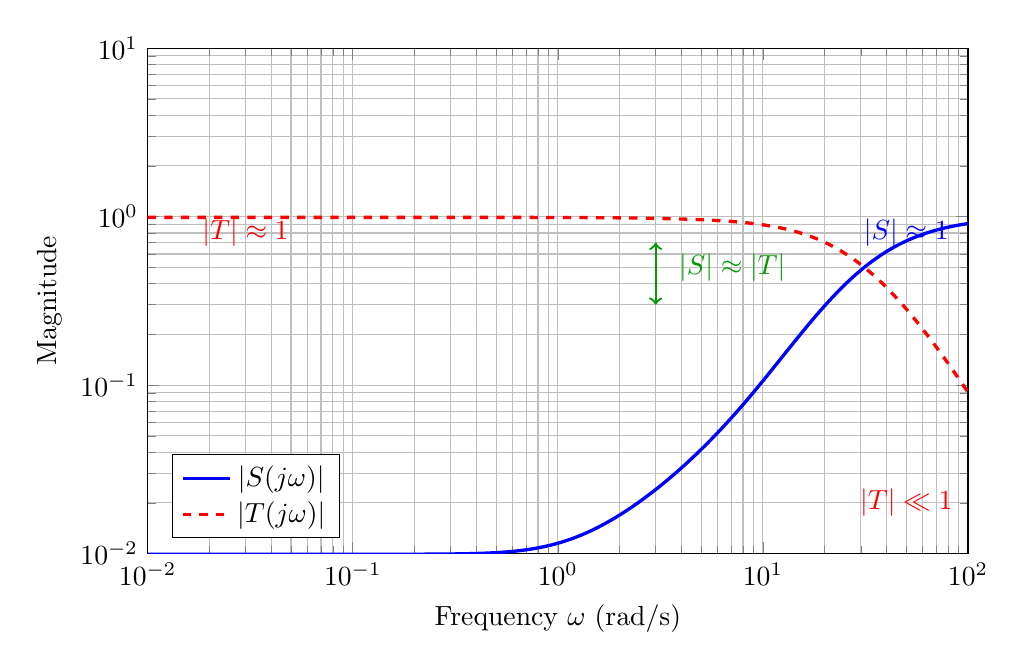
\begin{tikzpicture}
\begin{semilogyaxis}[
    width=12cm,
    height=8cm,
    xlabel={Frequency $\omega$ (rad/s)},
    ylabel={Magnitude},
    xmin=0.01, xmax=100,
    ymin=0.01, ymax=10,
    grid=both,
    legend pos=south west,
    xmode=log,
    domain=0.01:100,
    samples=200
]

% Loop gain L = 100/(1 + s/1)(1 + s/10)
% |L(jw)| = 100/sqrt((1+w^2)(1+w^2/100))

% S = 1/(1+L)
\addplot[blue, very thick] {1/sqrt((1 + 100/sqrt((1+x^2)*(1+x^2/100)))^2 + (100*x*(1/sqrt((1+x^2)*(1+x^2/100)))/(sqrt((1+x^2)*(1+x^2/100))))^2)};
\addlegendentry{$|S(j\omega)|$}

% T = L/(1+L) - approximation for visualization
\addplot[red, very thick, dashed] {1 - 1/sqrt((1 + 100/sqrt((1+x^2)*(1+x^2/100)))^2 + (100*x*(1/sqrt((1+x^2)*(1+x^2/100)))/(sqrt((1+x^2)*(1+x^2/100))))^2)};
\addlegendentry{$|T(j\omega)|$}

% Crossover frequency annotation
\draw[<->, thick, green!60!black] (axis cs:3,0.3) -- (axis cs:3,0.7);
\node[right, green!60!black] at (axis cs:3.5,0.5) {$|S| \approx |T|$};

% Low frequency region
\node[blue] at (axis cs:0.03,0.02) {$|S| \ll 1$};
\node[red] at (axis cs:0.03,0.8) {$|T| \approx 1$};

% High frequency region
\node[blue] at (axis cs:50,0.8) {$|S| \approx 1$};
\node[red] at (axis cs:50,0.02) {$|T| \ll 1$};

\end{semilogyaxis}
\end{tikzpicture}
\caption{Bode magnitude plots of sensitivity $S(j\omega)$ and complementary sensitivity $T(j\omega)$. At low frequencies where loop gain is high, $|S|$ is small (good disturbance rejection) and $|T| \approx 1$ (good tracking). At high frequencies, the roles reverse.}
\label{fig:s_t_bode}
\end{figure}

\subsection{Design Implications of S + T = 1}

The constraint $S + T = 1$ means that feedback design involves allocating the ``sensitivity budget'' across frequency. At low frequencies, the designer should make $|S| \ll 1$ to achieve good disturbance rejection and reference tracking accuracy, which requires high loop gain $|L| \gg 1$. At high frequencies, the goal shifts to making $|T| \ll 1$ to attenuate sensor noise, necessitating low loop gain $|L| \ll 1$. The crossover region, where the loop gain transitions from high to low values, must be designed carefully to ensure adequate stability margins---typically a phase margin greater than $30°$ and a gain margin exceeding $6$ dB.

The frequency at which $|L(j\omega_c)| = 1$ is called the \textit{crossover frequency} or \textit{bandwidth}. At this frequency, $|S| = |T| = 1/\sqrt{2} \approx 0.707$ (assuming $L$ crosses with $-90°$ phase).

\subsection{Noise and Disturbance: The Complete Picture}

From equation \eqref{eq:complete_output}, the complete output is:
\begin{equation}
Y = T \cdot R + G \cdot S \cdot D - T \cdot N
\end{equation}

This reveals the fundamental tradeoffs:
\begin{enumerate}
\item Making $T$ large (for tracking) amplifies noise $N$
\item Making $S$ small (for disturbance rejection) requires high loop gain, which also makes $T$ large
\item At high frequencies, we want $T$ small to reject noise, but this means $S \to 1$ and disturbance rejection is lost
\end{enumerate}

The art of control design is managing these tradeoffs across the frequency spectrum.

%=============================================================================
\section{Practical Experiment: Motor Speed Control with Disturbance Rejection}
\label{sec:practical_experiment}
%=============================================================================

In this laboratory experiment, we construct a motor speed control system and quantitatively measure the disturbance rejection provided by feedback. The experiment dramatically demonstrates why feedback is essential for maintaining performance under varying load conditions.

\subsection{Apparatus and Equipment}

The experiment requires a DC motor with optical encoder, such as the Pololu 37D metal gearmotor with 64 CPR encoder, which provides both the actuator and the velocity feedback signal. An Arduino Uno or compatible microcontroller serves as the digital controller, executing the control algorithm and communicating with the host computer. The L298N dual H-bridge motor driver interfaces between the low-power Arduino outputs and the motor's power requirements, while a 12V DC power supply provides the necessary electrical energy. An adjustable friction brake, constructed as described below, allows the application of controlled load disturbances. A multimeter with tachometer function may optionally be used to verify encoder-based speed measurements. Finally, a computer with the Arduino IDE and Serial Plotter enables programming, data acquisition, and real-time visualization of the control system response.

\begin{figure}[htbp]
\centering
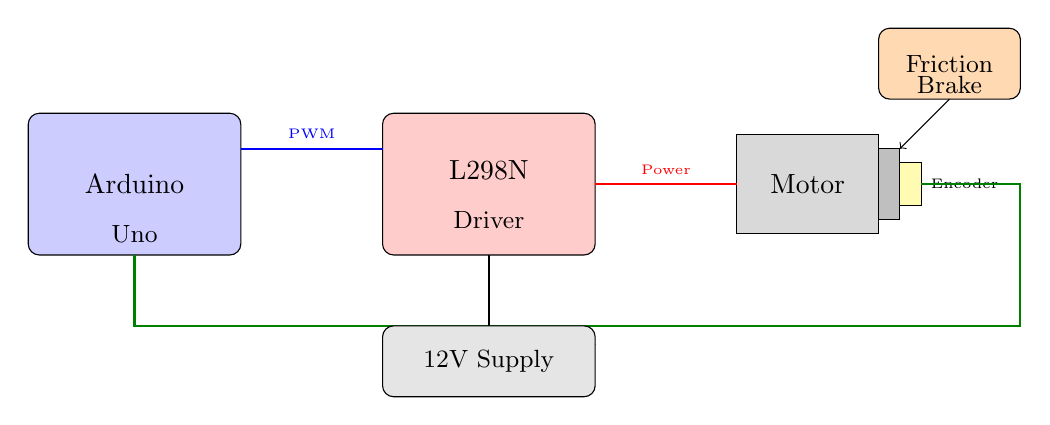
\begin{tikzpicture}[scale=0.9]
    % Arduino
    \draw[fill=blue!20, rounded corners] (0,0) rectangle (3,2);
    \node at (1.5,1) {Arduino};
    \node[font=\small] at (1.5,0.3) {Uno};

    % Motor driver
    \draw[fill=red!20, rounded corners] (5,0) rectangle (8,2);
    \node at (6.5,1.2) {L298N};
    \node[font=\small] at (6.5,0.5) {Driver};

    % Motor
    \draw[fill=gray!30] (10,0.3) rectangle (12,1.7);
    \node at (11,1) {Motor};
    \draw[fill=gray!50] (12,0.5) rectangle (12.3,1.5);

    % Encoder disc
    \draw[fill=yellow!30] (12.3,0.7) rectangle (12.6,1.3);
    \node[font=\tiny, right] at (12.6,1) {Encoder};

    % Brake
    \draw[fill=orange!30, rounded corners] (12,2.2) rectangle (14,3.2);
    \node[font=\small] at (13,2.7) {Friction};
    \node[font=\small] at (13,2.4) {Brake};
    \draw[->] (13,2.2) -- (12.3,1.5);

    % Connections
    \draw[thick, blue] (3,1.5) -- (5,1.5);
    \node[above, font=\tiny, blue] at (4,1.5) {PWM};

    \draw[thick, red] (8,1) -- (10,1);
    \node[above, font=\tiny, red] at (9,1) {Power};

    \draw[thick, green!50!black] (12.6,1) -- (14,1) -- (14,-1) -- (1.5,-1) -- (1.5,0);
    \node[below, font=\tiny, green!50!black] at (7,-1) {Encoder feedback};

    % Power supply
    \draw[fill=gray!20, rounded corners] (5,-2) rectangle (8,-1);
    \node[font=\small] at (6.5,-1.5) {12V Supply};
    \draw[thick] (6.5,-1) -- (6.5,0);

\end{tikzpicture}
\caption{Experimental setup for motor speed control with disturbance rejection measurement.}
\label{fig:experiment_setup}
\end{figure}

\subsection{Constructing the Friction Brake}

To apply controlled, measurable disturbances, we construct a simple friction brake:

\begin{enumerate}
\item Attach a wooden dowel or aluminum disk (diameter 50-75 mm) to the motor shaft
\item Create a brake arm from spring steel or a stiff plastic strip
\item Mount a felt pad on the brake arm contact point
\item Use an adjustment screw to vary the brake pressure
\item Calibrate the brake by measuring motor current at various settings
\end{enumerate}

The brake provides a load torque disturbance that we can apply suddenly while the motor is running.

\subsection{Software Implementation}

The following Arduino code implements both open-loop and closed-loop control modes, allowing direct comparison.

\begin{lstlisting}[style=arduino, caption={Motor speed control with disturbance rejection measurement}]
// Motor Speed Control with Disturbance Rejection
// Chapter 9 Laboratory Experiment

// Pin definitions
const int PWM_PIN = 9;      // Motor PWM output
const int DIR_PIN = 8;      // Motor direction
const int ENC_A = 2;        // Encoder channel A (interrupt)
const int ENC_B = 3;        // Encoder channel B

// Encoder variables
volatile long encoderCount = 0;
const int CPR = 64;         // Counts per revolution
const int GEAR_RATIO = 50;  // Gearbox ratio

// Control parameters
float Kp = 2.0;             // Proportional gain
float Ki = 5.0;             // Integral gain
float setpoint = 60.0;      // Desired speed in RPM
float integral = 0;

// Timing
unsigned long lastTime = 0;
const int SAMPLE_TIME = 50; // ms

// Mode selection
bool closedLoop = true;     // Toggle via serial command

void setup() {
  Serial.begin(115200);
  pinMode(PWM_PIN, OUTPUT);
  pinMode(DIR_PIN, OUTPUT);
  pinMode(ENC_A, INPUT_PULLUP);
  pinMode(ENC_B, INPUT_PULLUP);

  attachInterrupt(digitalPinToInterrupt(ENC_A),
                  encoderISR, RISING);

  digitalWrite(DIR_PIN, HIGH);
  Serial.println("Motor Control Ready");
  Serial.println("Commands: 'o'=open-loop, 'c'=closed-loop");
}

void encoderISR() {
  if (digitalRead(ENC_B)) encoderCount++;
  else encoderCount--;
}

void loop() {
  // Check for serial commands
  if (Serial.available()) {
    char cmd = Serial.read();
    if (cmd == 'o') {
      closedLoop = false;
      integral = 0;
      Serial.println("Open-loop mode");
    } else if (cmd == 'c') {
      closedLoop = true;
      Serial.println("Closed-loop mode");
    }
  }

  unsigned long now = millis();
  if (now - lastTime >= SAMPLE_TIME) {
    // Calculate speed in RPM
    noInterrupts();
    long count = encoderCount;
    encoderCount = 0;
    interrupts();

    float dt = (now - lastTime) / 1000.0;
    float rpm = (count * 60.0) / (CPR * GEAR_RATIO * dt);
    lastTime = now;

    int pwmOut;

    if (closedLoop) {
      // PI Controller
      float error = setpoint - rpm;
      integral += error * dt;
      integral = constrain(integral, -50, 50);

      float output = Kp * error + Ki * integral;
      pwmOut = constrain(128 + output, 0, 255);
    } else {
      // Open-loop: fixed PWM
      pwmOut = 128; // Nominally produces ~60 RPM
    }

    analogWrite(PWM_PIN, pwmOut);

    // Output for Serial Plotter
    Serial.print("Setpoint:");
    Serial.print(setpoint);
    Serial.print(",Speed:");
    Serial.print(rpm);
    Serial.print(",PWM:");
    Serial.println(pwmOut);
  }
}
\end{lstlisting}

\subsection{Experimental Procedure}

\begin{enumerate}
\item \textbf{Baseline measurement:} Run the motor in closed-loop mode with no brake applied. Record the steady-state speed and its variation.

\item \textbf{Open-loop disturbance response:}
\begin{enumerate}
    \item Switch to open-loop mode ('o' command)
    \item Allow speed to stabilize
    \item Apply brake suddenly; record the speed drop $\Delta\omega_{OL}$
    \item Release brake; verify return to original speed
    \item Repeat 5 times; calculate mean and standard deviation
\end{enumerate}

\item \textbf{Closed-loop disturbance response:}
\begin{enumerate}
    \item Switch to closed-loop mode ('c' command)
    \item Apply the same brake setting
    \item Record the speed drop $\Delta\omega_{CL}$
    \item Observe the recovery time to steady-state
    \item Repeat 5 times; calculate statistics
\end{enumerate}

\item \textbf{Disturbance rejection ratio:} Calculate:
\begin{equation}
\text{DRR} = \frac{\Delta\omega_{OL}}{\Delta\omega_{CL}}
\end{equation}

\item \textbf{Vary controller gain:} Repeat measurements with different $K_p$ values (1, 2, 5, 10) and plot DRR versus loop gain.
\end{enumerate}

\subsection{Expected Results and Analysis}

Table~\ref{tab:drr_results} shows typical experimental results for this apparatus.

\begin{table}[htbp]
\centering
\caption{Typical Disturbance Rejection Measurements}
\label{tab:drr_results}
\begin{tabular}{lccc}
\toprule
\textbf{Mode} & \textbf{Speed Drop} & \textbf{Recovery Time} & \textbf{DRR} \\
\midrule
Open-loop ($K_p = 0$) & 15.2 RPM & N/A & 1.0 (ref) \\
Closed-loop ($K_p = 1$) & 5.8 RPM & 0.8 s & 2.6 \\
Closed-loop ($K_p = 2$) & 3.1 RPM & 0.5 s & 4.9 \\
Closed-loop ($K_p = 5$) & 1.4 RPM & 0.3 s & 10.9 \\
Closed-loop ($K_p = 10$) & 0.8 RPM & 0.2 s & 19.0 \\
\bottomrule
\end{tabular}
\end{table}

The disturbance rejection ratio increases approximately linearly with loop gain, confirming the theoretical prediction $\text{DRR} \approx 1 + L(0)$ where $L(0)$ is the DC loop gain.

\begin{figure}[htbp]
\centering
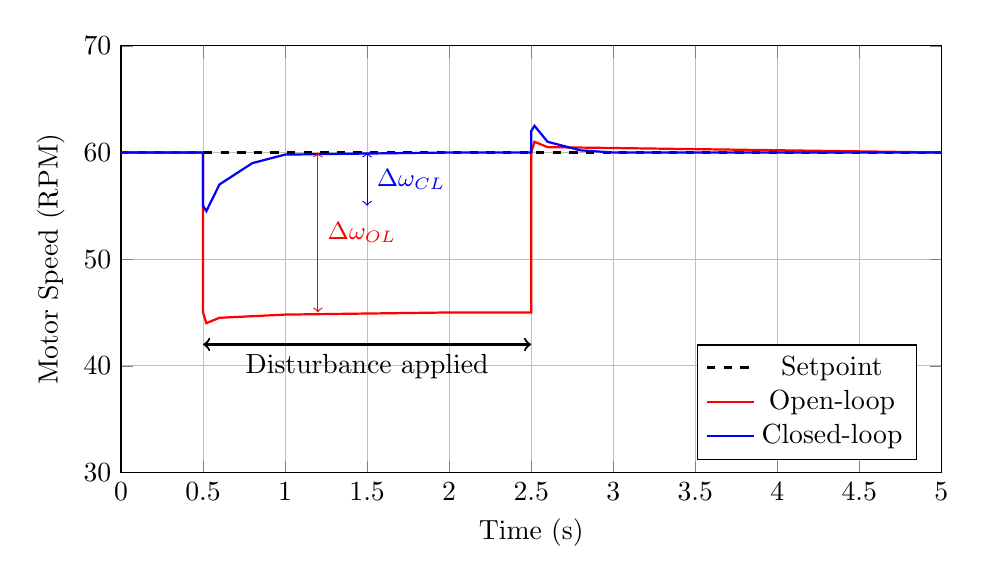
\begin{tikzpicture}
\begin{axis}[
    width=12cm,
    height=7cm,
    xlabel={Time (s)},
    ylabel={Motor Speed (RPM)},
    xmin=0, xmax=5,
    ymin=30, ymax=70,
    grid=both,
    legend pos=south east
]

% Setpoint
\addplot[black, dashed, very thick] coordinates {(0,60) (5,60)};
\addlegendentry{Setpoint}

% Open-loop response
\addplot[red, thick] coordinates {
    (0,60) (0.5,60) (0.5,45) (0.52,44) (0.6,44.5) (1,44.8)
    (2,45) (2.5,45) (2.5,60) (2.52,61) (2.6,60.5) (5,60)
};
\addlegendentry{Open-loop}

% Closed-loop response
\addplot[blue, thick] coordinates {
    (0,60) (0.5,60) (0.5,55) (0.52,54.5) (0.6,57) (0.8,59)
    (1,59.8) (2,60) (2.5,60) (2.5,62) (2.52,62.5) (2.6,61)
    (2.8,60.2) (3,60) (5,60)
};
\addlegendentry{Closed-loop}

% Disturbance annotation
\draw[<->, thick] (0.5,42) -- (2.5,42);
\node[below] at (1.5,42) {Disturbance applied};

% Speed drop annotations
\draw[<->, red] (1.2,45) -- (1.2,60);
\node[right, red, font=\small] at (1.2,52.5) {$\Delta\omega_{OL}$};

\draw[<->, blue] (1.5,55) -- (1.5,60);
\node[right, blue, font=\small] at (1.5,57.5) {$\Delta\omega_{CL}$};

\end{axis}
\end{tikzpicture}
\caption{Comparison of open-loop and closed-loop response to a load disturbance. The closed-loop system shows much smaller speed deviation and actively returns to the setpoint.}
\label{fig:disturbance_comparison}
\end{figure}

\subsection{Discussion Questions}

\begin{enumerate}
\item Why does higher loop gain provide better disturbance rejection but also faster recovery?

\item At what $K_p$ value did you observe oscillation or instability? Relate this to the stability margins.

\item How would integral action ($K_i > 0$) affect the steady-state disturbance rejection?

\item In industrial applications, why might we not simply use arbitrarily high gain?
\end{enumerate}

%=============================================================================
\section{Worked Examples}
\label{sec:worked_examples}
%=============================================================================

\begin{example}[Sensitivity Calculation: Open-Loop vs. Closed-Loop]
\label{ex:sensitivity_comparison}
An amplifier has nominal gain $A = 1000$ with $\pm 20\%$ variation. Calculate the output variation for:
\begin{enumerate}[(a)]
\item Open-loop operation
\item Closed-loop with feedback factor $\beta = 0.099$
\end{enumerate}

\textbf{Solution:}

\textbf{(a) Open-loop:}
The output is $V_{out} = A \cdot V_{in}$. With $\Delta A / A = \pm 0.20$:
\begin{equation}
\frac{\Delta V_{out}}{V_{out}} = \frac{\Delta A}{A} = \pm 20\%
\end{equation}

\textbf{(b) Closed-loop:}
The closed-loop gain is:
\begin{equation}
A_f = \frac{A}{1 + A\beta} = \frac{1000}{1 + 1000 \times 0.099} = \frac{1000}{100} = 10
\end{equation}

The sensitivity is:
\begin{equation}
S^A_{A_f} = \frac{1}{1 + A\beta} = \frac{1}{100} = 0.01
\end{equation}

Therefore:
\begin{equation}
\frac{\Delta A_f}{A_f} = S^A_{A_f} \cdot \frac{\Delta A}{A} = 0.01 \times (\pm 0.20) = \pm 0.2\%
\end{equation}

\textbf{Conclusion:} Feedback reduces the output variation from $\pm 20\%$ to $\pm 0.2\%$, a 100:1 improvement corresponding to the loop gain of 99.
\end{example}

\begin{example}[Closed-Loop Gain with Parameter Variations]
\label{ex:gain_variation}
A control system has nominal parameters consisting of a controller gain $C = 20$, a plant gain $G = 5$ (nominal) that can range from $3$ to $8$, and a sensor with unity gain $H = 1$.

Find the range of closed-loop transfer function $T = GC/(1+GCH)$.

\textbf{Solution:}

Nominal loop gain: $L = GCH = 5 \times 20 \times 1 = 100$

Nominal closed-loop gain:
\begin{equation}
T_{nom} = \frac{GC}{1+L} = \frac{100}{101} = 0.990
\end{equation}

With $G = 3$ (minimum):
\begin{equation}
L_{min} = 60, \quad T_{min} = \frac{60}{61} = 0.984
\end{equation}

With $G = 8$ (maximum):
\begin{equation}
L_{max} = 160, \quad T_{max} = \frac{160}{161} = 0.994
\end{equation}

\textbf{Range of $T$:} $[0.984, 0.994]$

While $G$ varies by a factor of $8/3 = 2.67$ (167\%), the closed-loop gain $T$ varies only from $0.984$ to $0.994$, a range of $\pm 0.5\%$ about the nominal value. This dramatic reduction in variability is the power of high-gain feedback.
\end{example}

\begin{example}[Designing for Specified Sensitivity]
\label{ex:design_sensitivity}
A plant has transfer function $G(s) = K/(s+1)$ where $K$ can vary by $\pm 25\%$ from its nominal value. Design a proportional controller $C(s) = K_c$ such that the DC closed-loop gain varies by no more than $\pm 1\%$.

\textbf{Solution:}

At DC ($s = 0$), the plant gain is $G(0) = K$. For unity feedback:
\begin{equation}
T(0) = \frac{K_c K}{1 + K_c K}
\end{equation}

The sensitivity at DC is:
\begin{equation}
S^K_{T(0)} = \frac{1}{1 + K_c K}
\end{equation}

For the closed-loop gain to vary by $\pm 1\%$ when $K$ varies by $\pm 25\%$:
\begin{equation}
\left|\frac{\Delta T}{T}\right| = S^K_{T(0)} \cdot \left|\frac{\Delta K}{K}\right| \leq 0.01
\end{equation}

\begin{equation}
\frac{1}{1 + K_c K} \times 0.25 \leq 0.01
\end{equation}

\begin{equation}
1 + K_c K \geq 25
\end{equation}

\begin{equation}
K_c K \geq 24
\end{equation}

If the nominal plant gain is $K = 2$:
\begin{equation}
K_c \geq \frac{24}{2} = 12
\end{equation}

\textbf{Design choice:} $K_c = 15$ provides margin. This yields a loop gain of $L(0) = 30$, a sensitivity of $S = 1/31 = 0.032$, and a closed-loop variation of $0.032 \times 25\% = 0.8\%$, which satisfies the specification of being less than $1\%$.
\end{example}

\begin{example}[Disturbance Rejection Analysis]
\label{ex:disturbance_rejection}
Consider a velocity control system with:
\begin{equation}
G(s) = \frac{10}{s + 2}, \quad C(s) = 5, \quad H(s) = 1
\end{equation}

A step disturbance of magnitude $D_0 = 0.5$ enters at the plant input. Find:
\begin{enumerate}[(a)]
\item The steady-state output deviation due to the disturbance
\item The disturbance rejection ratio compared to open-loop
\end{enumerate}

\textbf{Solution:}

\textbf{(a) Steady-state disturbance effect:}

The transfer function from disturbance to output is:
\begin{equation}
G_{YD}(s) = \frac{G(s)}{1 + G(s)C(s)H(s)} = \frac{\frac{10}{s+2}}{1 + \frac{50}{s+2}} = \frac{10}{s + 2 + 50} = \frac{10}{s + 52}
\end{equation}

For a step disturbance $D(s) = D_0/s = 0.5/s$:
\begin{equation}
Y_d(s) = G_{YD}(s) \cdot D(s) = \frac{10}{s+52} \cdot \frac{0.5}{s} = \frac{5}{s(s+52)}
\end{equation}

Using the final value theorem:
\begin{equation}
y_d(\infty) = \lim_{s \to 0} s \cdot Y_d(s) = \lim_{s \to 0} \frac{5}{s + 52} = \frac{5}{52} = 0.096
\end{equation}

\textbf{(b) Disturbance rejection ratio:}

In open-loop (no feedback, $C = 0$ or loop broken):
\begin{equation}
Y_{d,OL}(s) = G(s) D(s) = \frac{10}{s+2} \cdot \frac{0.5}{s}
\end{equation}

\begin{equation}
y_{d,OL}(\infty) = \lim_{s \to 0} \frac{5}{s+2} = \frac{5}{2} = 2.5
\end{equation}

Disturbance rejection ratio:
\begin{equation}
\text{DRR} = \frac{y_{d,OL}(\infty)}{y_d(\infty)} = \frac{2.5}{0.096} = 26
\end{equation}

This equals $1 + L(0) = 1 + 50/2 = 26$, confirming the theory.
\end{example}

\begin{example}[Operational Amplifier: Why Feedback Makes Gain Predictable]
\label{ex:opamp}
An operational amplifier has open-loop gain $A_{OL} = 10^5$ with a temperature coefficient of $-3000$ ppm/°C over the standard commercial operating range of $0°C$ to $70°C$.

Design a non-inverting amplifier with nominal gain of 10 using $0.1\%$ tolerance resistors. Compare the total gain uncertainty for open-loop versus closed-loop operation.

\textbf{Solution:}

\begin{figure}[htbp]
\centering
\begin{circuitikz}[american]
    % Op-amp
    \draw (0,0) node[op amp, yscale=1] (opamp) {};

    % Input
    \draw (opamp.+) -- ++(-1,0) node[left] {$V_{in}$};

    % Feedback network
    \draw (opamp.-) -- ++(0,-1) coordinate(fb);
    \draw (fb) to[R, l=$R_1$] ++(0,-1.5) node[ground] {};
    \draw (fb) -- ++(-0.5,0) -- ++(0,-0.3);
    \draw (opamp.out) -- ++(1,0) coordinate(out);
    \draw (out) -- ++(0,-1.5) to[R, l=$R_2$] (fb |- 0,-1.5) -- (fb);

    % Output
    \draw (out) -- ++(0.5,0) node[right] {$V_{out}$};

    % Component values
    \node[below right] at (opamp.south) {$A_{OL} = 10^5$};
\end{circuitikz}
\caption{Non-inverting amplifier configuration for Example~\ref{ex:opamp}.}
\end{figure}

\textbf{Feedback factor:}
For gain of 10, we need $1 + R_2/R_1 = 10$, so $R_2/R_1 = 9$.

Choose $R_1 = \SI{1}{k\Omega}$, $R_2 = \SI{9}{k\Omega}$, both $0.1\%$ tolerance.

\begin{equation}
\beta = \frac{R_1}{R_1 + R_2} = \frac{1}{10} = 0.1
\end{equation}

\textbf{Open-loop gain variation:}

Temperature change: $\Delta T = 70°C$

Gain change: $\Delta A_{OL}/A_{OL} = -3000 \times 10^{-6} \times 70 = -0.21 = -21\%$

\textbf{Closed-loop analysis:}

Loop gain: $L = A_{OL} \cdot \beta = 10^5 \times 0.1 = 10^4$

Closed-loop gain:
\begin{equation}
A_{CL} = \frac{A_{OL}}{1 + A_{OL}\beta} = \frac{10^5}{1 + 10^4} \approx \frac{10^5}{10^4} = 10
\end{equation}

More precisely:
\begin{equation}
A_{CL} = \frac{10^5}{10001} = 9.999
\end{equation}

\textbf{Sensitivity to open-loop gain:}
\begin{equation}
S^{A_{OL}}_{A_{CL}} = \frac{1}{1 + L} = \frac{1}{10001} \approx 10^{-4}
\end{equation}

Effect of $21\%$ open-loop variation:
\begin{equation}
\frac{\Delta A_{CL}}{A_{CL}} = 10^{-4} \times 0.21 = 0.0021\% = 21 \text{ ppm}
\end{equation}

\textbf{Sensitivity to resistor ratio:}

The closed-loop gain depends on $\beta = R_1/(R_1+R_2)$, which depends on the resistor ratio $R_2/R_1$:
\begin{equation}
A_{CL} \approx \frac{1}{\beta} = 1 + \frac{R_2}{R_1}
\end{equation}

With $0.1\%$ resistors, the ratio $R_2/R_1$ can vary by approximately $\pm 0.2\%$ (root-sum-square of the two resistor tolerances):
\begin{equation}
\frac{\Delta A_{CL}}{A_{CL}} \approx \frac{\Delta(R_2/R_1)}{1 + R_2/R_1} = \frac{0.002 \times 9}{10} = 0.18\%
\end{equation}

\textbf{Summary:}
\begin{center}
\begin{tabular}{lc}
\toprule
\textbf{Error Source} & \textbf{Contribution} \\
\midrule
Open-loop gain (temperature) & 21 ppm \\
Resistor ratio ($0.1\%$ resistors) & 1800 ppm \\
\midrule
\textbf{Total (RSS)} & $\approx$ \textbf{1800 ppm = 0.18\%} \\
\bottomrule
\end{tabular}
\end{center}

Without feedback, gain would vary by $21\%$. With feedback, the variation is $0.18\%$, dominated by the resistor tolerance---not the amplifier. This is exactly Black's vision: the system performance is determined by the passive feedback components, not the active device.
\end{example}

\begin{example}[S + T = 1 and the Noise-Disturbance Tradeoff]
\label{ex:tradeoff}
A control system has loop transfer function:
\begin{equation}
L(s) = \frac{1000}{(s+1)(s+10)}
\end{equation}

Calculate $|S(j\omega)|$ and $|T(j\omega)|$ at:
\begin{enumerate}[(a)]
\item $\omega = 0.1$ rad/s (low frequency)
\item $\omega = 10$ rad/s (crossover region)
\item $\omega = 100$ rad/s (high frequency)
\end{enumerate}

Verify that $|S|^2 + |T|^2 \neq 1$ in general (but $S + T = 1$ always).

\textbf{Solution:}

\textbf{(a) $\omega = 0.1$ rad/s:}
\begin{equation}
L(j0.1) = \frac{1000}{(1+j0.1)(10+j0.1)} \approx \frac{1000}{10} = 100
\end{equation}

\begin{equation}
S = \frac{1}{1+L} \approx \frac{1}{101} = 0.0099, \quad |S| = 0.0099
\end{equation}

\begin{equation}
T = \frac{L}{1+L} \approx \frac{100}{101} = 0.990, \quad |T| = 0.990
\end{equation}

At low frequency: excellent disturbance rejection ($|S| \ll 1$), excellent tracking ($|T| \approx 1$).

\textbf{(b) $\omega = 10$ rad/s:}
\begin{equation}
L(j10) = \frac{1000}{(1+j10)(10+j10)} = \frac{1000}{(1+j10)(10)(1+j)}
\end{equation}

\begin{equation}
|L(j10)| = \frac{1000}{10 \times \sqrt{101} \times \sqrt{2}} = \frac{1000}{142} = 7.04
\end{equation}

\begin{equation}
|S| = \frac{1}{|1 + L|} \approx \frac{1}{8} = 0.125
\end{equation}

\begin{equation}
|T| = \frac{|L|}{|1+L|} \approx \frac{7}{8} = 0.875
\end{equation}

At crossover: moderate disturbance rejection and tracking.

\textbf{(c) $\omega = 100$ rad/s:}
\begin{equation}
|L(j100)| = \frac{1000}{\sqrt{1+10000} \times \sqrt{100+10000}} = \frac{1000}{100 \times 100} = 0.1
\end{equation}

\begin{equation}
|S| \approx \frac{1}{1.1} = 0.91, \quad |T| \approx \frac{0.1}{1.1} = 0.091
\end{equation}

At high frequency: poor disturbance rejection ($|S| \approx 1$), good noise rejection ($|T| \ll 1$).

\textbf{Verification of $S + T = 1$:}

Note that $|S|^2 + |T|^2 \neq 1$ because $S$ and $T$ are complex numbers. However:
\begin{equation}
S(s) + T(s) = \frac{1}{1+L(s)} + \frac{L(s)}{1+L(s)} = 1
\end{equation}

This is an algebraic identity that holds for all $s$, including $s = j\omega$. The magnitude inequality $|S| + |T| \neq 1$ (in general) is a consequence of complex addition.
\end{example}

%=============================================================================
\section{Block Diagram: Disturbance Analysis}
\label{sec:block_diagram}
%=============================================================================

\begin{figure}[htbp]
\centering
\begin{tikzpicture}[auto, node distance=2.2cm, >=latex', scale=0.85, transform shape]

    % Title
    \node[font=\large\bfseries] at (5,4) {Standard Feedback Control System with Disturbance};

    % Main blocks
    \node[draw, circle, minimum size=0.8cm, thick] (sum1) at (0,0) {$\Sigma$};
    \node[draw, rectangle, minimum width=2cm, minimum height=1.2cm, thick, fill=blue!10] (C) at (3,0) {$C(s)$};
    \node[draw, circle, minimum size=0.8cm, thick] (sum2) at (6,0) {$\Sigma$};
    \node[draw, rectangle, minimum width=2cm, minimum height=1.2cm, thick, fill=green!10] (G) at (9,0) {$G(s)$};

    % Labels
    \node[below=0.1cm, font=\small] at (C.south) {Controller};
    \node[below=0.1cm, font=\small] at (G.south) {Plant};

    % Input
    \node[left=1.5cm] (R) at (sum1) {$R(s)$};
    \node[above=0.1cm, font=\small] at (R.north) {Reference};

    % Disturbance
    \node[above=1.2cm] (D) at (sum2) {$D(s)$};
    \node[right=0.1cm, font=\small] at (D.east) {Disturbance};

    % Output
    \node[right=2cm] (Y) at (G) {$Y(s)$};
    \node[above=0.1cm, font=\small] at (Y.north) {Output};

    % Feedback
    \node[draw, rectangle, minimum width=1.5cm, minimum height=0.8cm, thick, fill=orange!10] (H) at (5,-2.5) {$H(s)$};
    \node[below=0.1cm, font=\small] at (H.south) {Sensor};

    % Connections
    \draw[->, thick] (R) -- (sum1);
    \draw[->, thick] (sum1) -- node[above] {$E(s)$} (C);
    \draw[->, thick] (C) -- node[above] {$U(s)$} (sum2);
    \draw[->, thick] (D) -- (sum2);
    \draw[->, thick] (sum2) -- (G);
    \draw[->, thick] (G) -- (Y);

    % Feedback path
    \draw[->, thick] (11,0) -- (11,-2.5) -- (H);
    \draw[->, thick] (H) -- (0,-2.5) -- (sum1);

    % Signs
    \node[font=\small] at (-0.35,0.25) {$+$};
    \node[font=\small] at (-0.35,-0.35) {$-$};
    \node[font=\small] at (5.65,0.25) {$+$};
    \node[font=\small] at (6.35,0.25) {$+$};

    % Transfer function box
    \draw[dashed, thick, rounded corners] (-2,-4) rectangle (13,3.2);

    % Key equations box
    \node[draw, fill=yellow!20, rounded corners, text width=5.5cm, align=left, font=\small] at (10.5,-3.5) {
        \textbf{Key Transfer Functions:}\\[3pt]
        $T = \dfrac{Y}{R} = \dfrac{GC}{1+GCH}$\\[6pt]
        $\dfrac{Y}{D} = \dfrac{G}{1+GCH} = G \cdot S$\\[6pt]
        $S = \dfrac{1}{1+L}, \quad L = GCH$
    };

\end{tikzpicture}
\caption{Complete feedback control system block diagram showing how disturbances enter at the plant input and are attenuated by the sensitivity function $S(s) = 1/(1+L(s))$.}
\label{fig:complete_block_diagram}
\end{figure}

%=============================================================================
\section{Summary}
\label{sec:summary}
%=============================================================================

This chapter has explored the fundamental role of feedback in reducing sensitivity to parameter variations and rejecting disturbances. The key concepts are:

\begin{enumerate}
\item \textbf{Historical foundation:} Harold Black's 1927 invention of the negative feedback amplifier solved the critical problem of amplifier gain drift in transcontinental telephone systems. By deliberately sacrificing gain, Black achieved unprecedented stability and linearity.

\item \textbf{Sensitivity function:} The function $S(s) = 1/(1+L(s))$ quantifies both the attenuation of disturbances entering at the plant input and the reduction in sensitivity to plant parameter variations.

\item \textbf{High loop gain benefit:} When $|L(j\omega)| \gg 1$, the sensitivity $|S(j\omega)| \ll 1$, providing excellent disturbance rejection and parameter insensitivity.

\item \textbf{Complementary sensitivity:} The function $T(s) = L(s)/(1+L(s))$ describes reference tracking and noise transmission. The fundamental constraint $S + T = 1$ means we cannot simultaneously minimize both.

\item \textbf{Frequency-dependent design:} Good design requires high loop gain at low frequencies (for disturbance rejection and tracking) and low loop gain at high frequencies (for noise rejection and stability).

\item \textbf{Practical verification:} Laboratory experiments with motor speed control demonstrate that disturbance rejection improves proportionally with loop gain, confirming theoretical predictions.
\end{enumerate}

The principles developed in this chapter---sensitivity reduction, disturbance rejection, and the $S + T = 1$ tradeoff---form the foundation for modern robust control design methods covered in subsequent chapters.

%=============================================================================
\section{Problems}
\label{sec:problems}
%=============================================================================

\begin{enumerate}
\item A unity feedback system has $G(s) = K/(s+5)$ and $C(s) = 10$.
\begin{enumerate}[(a)]
    \item Find the sensitivity $S^K_T$ at DC.
    \item If $K$ changes from 100 to 120, what is the percentage change in $T(0)$?
\end{enumerate}

\item For the system in Problem 1, a step disturbance of magnitude 2 enters at the plant input. Find:
\begin{enumerate}[(a)]
    \item The steady-state output deviation
    \item The disturbance rejection ratio compared to open-loop
\end{enumerate}

\item An operational amplifier with $A_{OL} = 50{,}000$ is used in an inverting configuration with $R_1 = \SI{1}{k\Omega}$ and $R_f = \SI{100}{k\Omega}$.
\begin{enumerate}[(a)]
    \item Calculate the ideal and actual closed-loop gain.
    \item Find the sensitivity of the closed-loop gain to $A_{OL}$.
    \item If $A_{OL}$ decreases by 50\% due to loading, what is the percentage change in closed-loop gain?
\end{enumerate}

\item Derive the transfer function from measurement noise $N(s)$ to output $Y(s)$ for the standard feedback configuration. Explain why high bandwidth (high $|T(j\omega)|$ at high frequencies) is undesirable from a noise perspective.

\item A cruise control system has plant $G(s) = 1/(10s+1)$ representing vehicle dynamics. Design a PI controller $C(s) = K_p + K_i/s$ such that:
\begin{enumerate}[(a)]
    \item The DC loop gain exceeds 100 (for disturbance rejection)
    \item The crossover frequency is approximately 1 rad/s
\end{enumerate}

\item Prove that for a general feedback system, the sensitivity of $T$ with respect to the feedback element $H$ is:
\begin{equation}
S^H_T = -\frac{L}{1+L} = -T
\end{equation}
Interpret this result: why is the sensitivity to $H$ approximately $-1$ when loop gain is high?

\item A temperature control system has plant $G(s) = 2/((s+0.1)(s+1))$. The plant gain can vary by $\pm 30\%$ due to heat exchanger fouling. Design a proportional controller to limit the closed-loop gain variation to $\pm 3\%$.

\item Using the Bode magnitude plot, sketch $|S(j\omega)|$ and $|T(j\omega)|$ for:
\begin{equation}
L(s) = \frac{100}{s(s/10 + 1)}
\end{equation}
Identify the crossover frequency and verify that $|S(j\omega_c)| \approx |T(j\omega_c)|$.

\item In the motor control experiment (Section~\ref{sec:practical_experiment}), derive a theoretical expression for the disturbance rejection ratio as a function of proportional gain $K_p$, assuming the motor transfer function is $G(s) = K_m/(s + a)$.

\item \textbf{Design project:} Implement the motor speed control experiment using an Arduino and any available DC motor with encoder. Measure the disturbance rejection ratio for at least 4 different controller gains. Plot DRR versus loop gain and compare with theoretical predictions.
\end{enumerate}

%=============================================================================
% References
%=============================================================================

\begin{thebibliography}{99}

\bibitem{black1934}
H. S. Black, ``Stabilized feedback amplifiers,'' \textit{Bell System Technical Journal}, vol. 13, no. 1, pp. 1--18, Jan. 1934.

\bibitem{bode1945}
H. W. Bode, \textit{Network Analysis and Feedback Amplifier Design}. New York: Van Nostrand, 1945.

\bibitem{nyquist1932}
H. Nyquist, ``Regeneration theory,'' \textit{Bell System Technical Journal}, vol. 11, no. 1, pp. 126--147, Jan. 1932.

\bibitem{franklin2015}
G. F. Franklin, J. D. Powell, and A. Emami-Naeini, \textit{Feedback Control of Dynamic Systems}, 7th ed. Upper Saddle River, NJ: Pearson, 2015.

\bibitem{astrom2021}
K. J. \r{A}str\"{o}m and R. M. Murray, \textit{Feedback Systems: An Introduction for Scientists and Engineers}, 2nd ed. Princeton, NJ: Princeton University Press, 2021.

\bibitem{dorf2017}
R. C. Dorf and R. H. Bishop, \textit{Modern Control Systems}, 13th ed. Upper Saddle River, NJ: Pearson, 2017.

\bibitem{skogestad2005}
S. Skogestad and I. Postlethwaite, \textit{Multivariable Feedback Control: Analysis and Design}, 2nd ed. Chichester, UK: Wiley, 2005.

\bibitem{mindell2002}
D. A. Mindell, \textit{Between Human and Machine: Feedback, Control, and Computing Before Cybernetics}. Baltimore, MD: Johns Hopkins University Press, 2002.

\end{thebibliography}

